\documentclass[aspectratio=169]{beamer}

\usepackage{graphicx}
\usepackage{polski}
\usepackage[utf8]{inputenc}

\title{OpenStack Cinder Deep Dive}
\author{Michał Dulko}
\date{August 4th, 2016}

\begin{document}

\begin{frame}
\titlepage
\end{frame}

\section{Main}

\begin{frame}
\frametitle{Cinder's Mission}
\pause
\begin{center}
    \huge To implement services and libraries to provide on-demand, self-service
    access to Block Storage resources via abstraction and automation on top of
    other block storage devices.
\end{center}

\end{frame}

\begin{frame}
    \frametitle{Cinder drivers}
    Cinder is an abstraction layer for around 80 storage backends:
    \begin{itemize}
        \item Open: LVM, GlusterFS, Ceph, NFS…
        \item Proprietary: NetApp, SolidFire, Dell, EMC, HPE, Fujitsu, Hitachi, IBM, Lenovo, VMWare, Violin, Quobyte, Scality, Tegile…
        \item Protocols: iSCSI, NFS, RBD, Fiber Channel, proprietary…
        \item Backup: Swift, RBD, GlusterFS, NFS, IBM TSM
    \end{itemize}
\end{frame}

\begin{frame}
    \frametitle{Required features}
    \begin{itemize}
        \item Volume Create/Delete
        \item Volume Attach/Detach
        \item Snapshot Create/Delete
        \item Create Volume from Snapshot
        \item Get Volume Stats
        \item Copy Image to Volume
        \item Copy Volume to Image
        \item Clone Volume
        \item Extend Volume
    \end{itemize}
\end{frame}

\begin{frame}
    \frametitle{Other/optional features}
    \begin{itemize}
        \pause
        \item Backups
        \begin{itemize}
            \item CPU bound!
            \item Depends on cinder-backup service
        \end{itemize}
        \pause
        \item Encryption
        \begin{itemize}
            \item Many restrictions 
        \end{itemize}
        \pause
        \item \emph{Replication}
        \begin{itemize}
            \item Low number of supporting drivers
            \item Replication v1 - single volume replication
            \item Replication v2 - backend-level replication
        \end{itemize}
        \pause
        \item \emph{Consistency groups and snapshots}
        \begin{itemize}
            \item Low number of supporting drivers
            \item Quite reliable
        \end{itemize}
        \pause
        \item \emph{QoS support}
        \begin{itemize}
            \item Moderate number of supporting drivers
        \end{itemize}
    \end{itemize}
\end{frame}

\begin{frame}
    \frametitle{Architecture (pre-Mitaka)}
    \begin{center}
        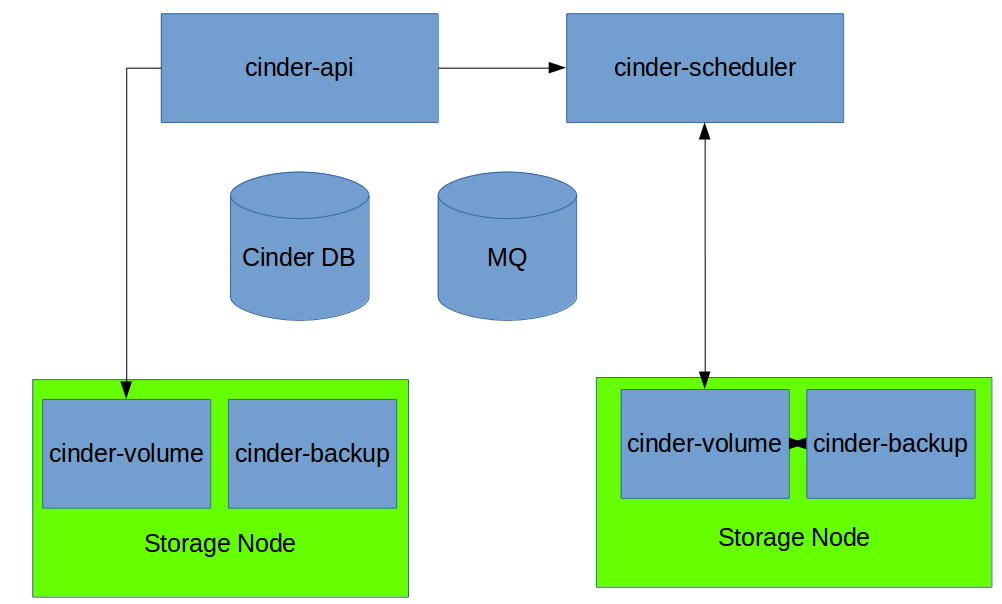
\includegraphics[height=6cm]{images/architecture-pre-mitaka.png}
    \end{center}
\end{frame}

\begin{frame}
    \frametitle{Architecture (since Mitaka)}
    \begin{center}
        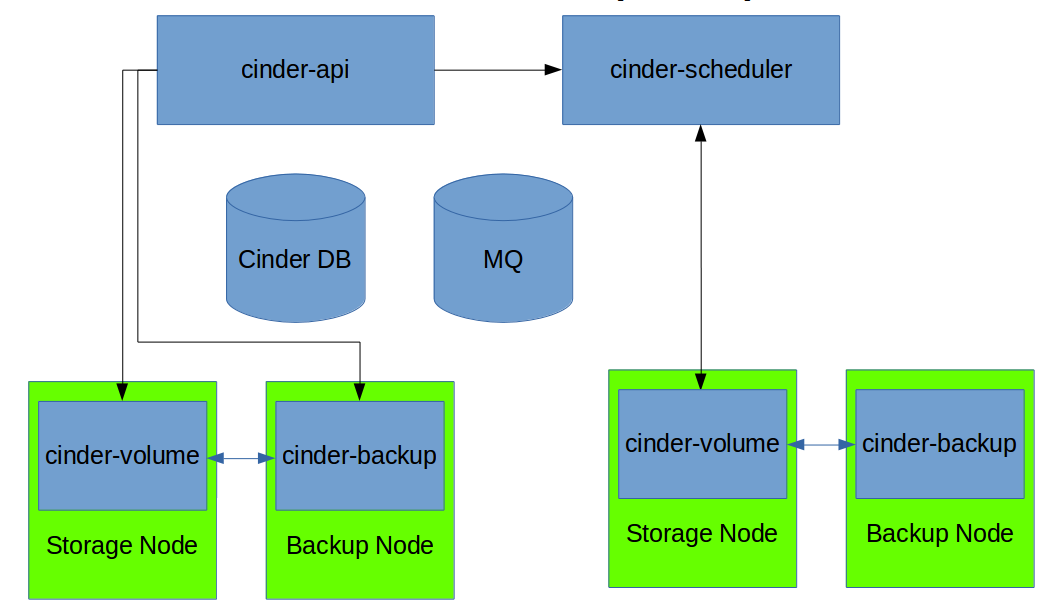
\includegraphics[height=6cm]{images/architecture-post-mitaka.png}
    \end{center}
\end{frame}

\begin{frame}
    \frametitle{Architecture}
    \begin{center}
        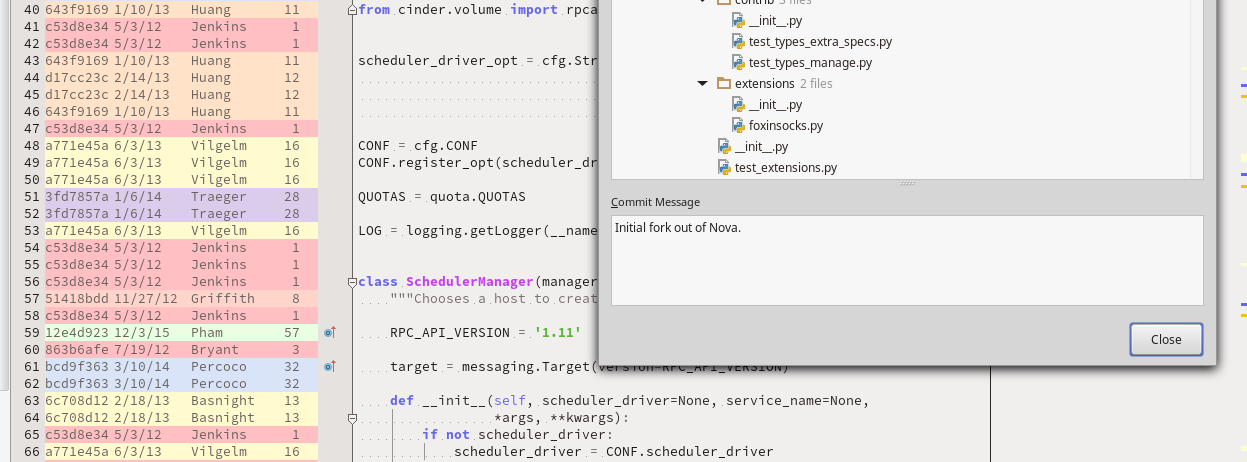
\includegraphics[width=\textwidth]{images/initial-fork.png}
    \end{center}
\end{frame}

\begin{frame}
    \frametitle{Architecture (non-LVM-backends)}
    \begin{center}
        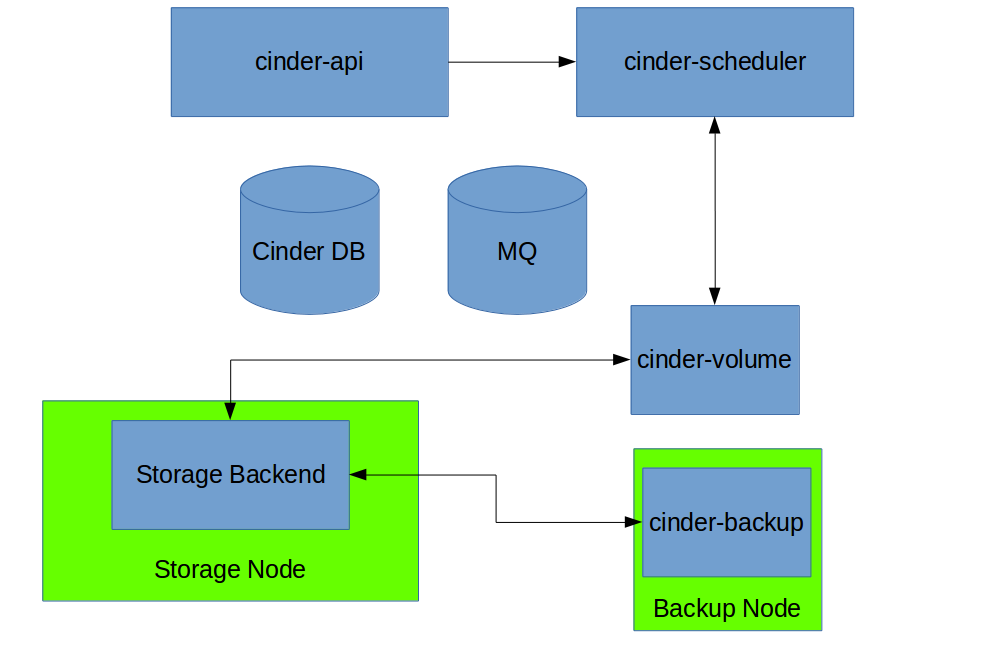
\includegraphics[height=6cm]{images/architecture-prop.png}
    \end{center}
\end{frame}

\begin{frame}
    \frametitle{Attach to VM or detach from VM}
    Complicated chain of internal REST API calls from Nova to Cinder.
    \pause
    \begin{center}
        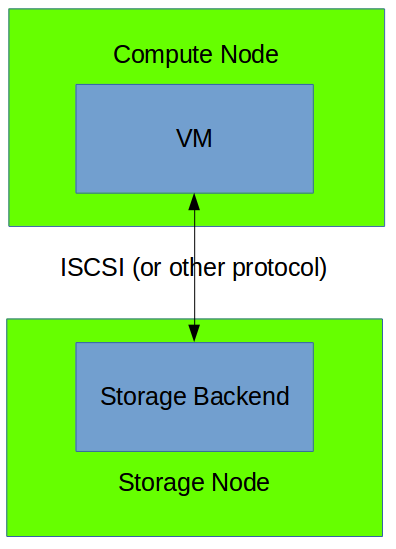
\includegraphics[height=5cm]{images/attached.png}
    \end{center}
\end{frame}

\begin{frame}
    \frametitle{Pitfalls}
    \begin{itemize}
        \pause
        \item cinder-scheduler is race-condition prone
        \begin{itemize}
            \item Nova's legacy
        \end{itemize}
        \pause
        \item multi-backend support
        \begin{itemize}
            \item It's like running multiple cinder-volume on one node
            \item Deployment without enabled\_backends option is deprecated in Newton
        \end{itemize}
        \pause
        \item Cinder usage outside of OpenStack
        \begin{itemize}
            \item python-brick-cinderclient-ext project 
            \item You'll still need DB (MySQL), MQ (RabbitMQ) and Keystone
        \end{itemize}
    \end{itemize}
\end{frame}

\begin{frame}
    \frametitle{Future}
    \begin{itemize}
        \item Replication v2.1
        \begin{itemize}
            \item replication of groups of volumes
        \end{itemize}
        \pause
        \item Ironic support
        \pause
        \item Volume multi-attach support
        \begin{itemize}
            \item Cinder's side is done… \pause since Liberty
            \item Still trying to figure out correct Nova-Cinder interactions
        \end{itemize}
        \pause
        \item Live upgrade support
        \begin{itemize}
            \item Experimental in Mitaka
            \item Hopefully Newton will officially support that
        \end{itemize}
        \pause
        \item cinder-volume service clustering AKA \emph{c-vol A/A HA support}
        \begin{itemize}
            \item Right now it is still risky to run multiple c-vols controlling a single storage backend
        \end{itemize}
    \end{itemize}
\end{frame}

\begin{frame}
    \begin{center}
        \huge Thank you!
    \end{center}
\end{frame}

\end{document}

